% Options for packages loaded elsewhere
\PassOptionsToPackage{unicode}{hyperref}
\PassOptionsToPackage{hyphens}{url}
\PassOptionsToPackage{dvipsnames,svgnames,x11names}{xcolor}
%
\documentclass[
  ignorenonframetext,
]{beamer}
\usepackage{pgfpages}
\setbeamertemplate{caption}[numbered]
\setbeamertemplate{caption label separator}{: }
\setbeamercolor{caption name}{fg=normal text.fg}
\beamertemplatenavigationsymbolsempty
% Prevent slide breaks in the middle of a paragraph
\widowpenalties 1 10000
\raggedbottom

\usepackage{amsmath,amssymb}
\usepackage{iftex}
\ifPDFTeX
  \usepackage[T1]{fontenc}
  \usepackage[utf8]{inputenc}
  \usepackage{textcomp} % provide euro and other symbols
\else % if luatex or xetex
  \usepackage{unicode-math}
  \defaultfontfeatures{Scale=MatchLowercase}
  \defaultfontfeatures[\rmfamily]{Ligatures=TeX,Scale=1}
\fi
\usepackage{lmodern}
\usetheme[]{AnnArbor}
\usecolortheme{dolphin}
\usefonttheme{structurebold}
\ifPDFTeX\else  
    % xetex/luatex font selection
\fi
% Use upquote if available, for straight quotes in verbatim environments
\IfFileExists{upquote.sty}{\usepackage{upquote}}{}
\IfFileExists{microtype.sty}{% use microtype if available
  \usepackage[]{microtype}
  \UseMicrotypeSet[protrusion]{basicmath} % disable protrusion for tt fonts
}{}
\makeatletter
\@ifundefined{KOMAClassName}{% if non-KOMA class
  \IfFileExists{parskip.sty}{%
    \usepackage{parskip}
  }{% else
    \setlength{\parindent}{0pt}
    \setlength{\parskip}{6pt plus 2pt minus 1pt}}
}{% if KOMA class
  \KOMAoptions{parskip=half}}
\makeatother
\usepackage{xcolor}
\newif\ifbibliography
\setlength{\emergencystretch}{3em} % prevent overfull lines
\setcounter{secnumdepth}{-\maxdimen} % remove section numbering


\providecommand{\tightlist}{%
  \setlength{\itemsep}{0pt}\setlength{\parskip}{0pt}}\usepackage{longtable,booktabs,array}
\usepackage{calc} % for calculating minipage widths
\usepackage{caption}
% Make caption package work with longtable
\makeatletter
\def\fnum@table{\tablename~\thetable}
\makeatother
\usepackage{graphicx}
\makeatletter
\def\maxwidth{\ifdim\Gin@nat@width>\linewidth\linewidth\else\Gin@nat@width\fi}
\def\maxheight{\ifdim\Gin@nat@height>\textheight\textheight\else\Gin@nat@height\fi}
\makeatother
% Scale images if necessary, so that they will not overflow the page
% margins by default, and it is still possible to overwrite the defaults
% using explicit options in \includegraphics[width, height, ...]{}
\setkeys{Gin}{width=\maxwidth,height=\maxheight,keepaspectratio}
% Set default figure placement to htbp
\makeatletter
\def\fps@figure{htbp}
\makeatother
% definitions for citeproc citations
\NewDocumentCommand\citeproctext{}{}
\NewDocumentCommand\citeproc{mm}{%
  \begingroup\def\citeproctext{#2}\cite{#1}\endgroup}
\makeatletter
 % allow citations to break across lines
 \let\@cite@ofmt\@firstofone
 % avoid brackets around text for \cite:
 \def\@biblabel#1{}
 \def\@cite#1#2{{#1\if@tempswa , #2\fi}}
\makeatother
\newlength{\cslhangindent}
\setlength{\cslhangindent}{1.5em}
\newlength{\csllabelwidth}
\setlength{\csllabelwidth}{3em}
\newenvironment{CSLReferences}[2] % #1 hanging-indent, #2 entry-spacing
 {\begin{list}{}{%
  \setlength{\itemindent}{0pt}
  \setlength{\leftmargin}{0pt}
  \setlength{\parsep}{0pt}
  % turn on hanging indent if param 1 is 1
  \ifodd #1
   \setlength{\leftmargin}{\cslhangindent}
   \setlength{\itemindent}{-1\cslhangindent}
  \fi
  % set entry spacing
  \setlength{\itemsep}{#2\baselineskip}}}
 {\end{list}}
\usepackage{calc}
\newcommand{\CSLBlock}[1]{\hfill\break\parbox[t]{\linewidth}{\strut\ignorespaces#1\strut}}
\newcommand{\CSLLeftMargin}[1]{\parbox[t]{\csllabelwidth}{\strut#1\strut}}
\newcommand{\CSLRightInline}[1]{\parbox[t]{\linewidth - \csllabelwidth}{\strut#1\strut}}
\newcommand{\CSLIndent}[1]{\hspace{\cslhangindent}#1}


% logo
\titlegraphic{
\includegraphics[width=4cm]{000_logos/logo-blue-vertical}}
\logo{\ifnum\thepage>1
\includegraphics[width=0.5cm]{000_logos/logo-blue-vertical}\fi}

% UMNG: Manual de image institucional

% Colors

% Umng
\definecolor{yellow}{HTML}{fdc600}
\definecolor{red}{HTML}{ee2a24}

% Estudios a Distancia
\definecolor{blue1}{HTML}{12245b}
\definecolor{blue2}{HTML}{767ca6}
\definecolor{blue3}{HTML}{cad2ec}

% Modify items
\setbeamercolor{palette primary}{bg=blue3}
\setbeamercolor{palette tertiary}{bg=blue1}
\setbeamercolor{frametitle}{bg=yellow}

% Hyperlinks
\hypersetup{
  linkcolor=red,
  citecolor=red
}

\makeatletter
\@ifpackageloaded{caption}{}{\usepackage{caption}}
\AtBeginDocument{%
\ifdefined\contentsname
  \renewcommand*\contentsname{Table of contents}
\else
  \newcommand\contentsname{Table of contents}
\fi
\ifdefined\listfigurename
  \renewcommand*\listfigurename{List of Figures}
\else
  \newcommand\listfigurename{List of Figures}
\fi
\ifdefined\listtablename
  \renewcommand*\listtablename{List of Tables}
\else
  \newcommand\listtablename{List of Tables}
\fi
\ifdefined\figurename
  \renewcommand*\figurename{Figure}
\else
  \newcommand\figurename{Figure}
\fi
\ifdefined\tablename
  \renewcommand*\tablename{Table}
\else
  \newcommand\tablename{Table}
\fi
}
\@ifpackageloaded{float}{}{\usepackage{float}}
\floatstyle{ruled}
\@ifundefined{c@chapter}{\newfloat{codelisting}{h}{lop}}{\newfloat{codelisting}{h}{lop}[chapter]}
\floatname{codelisting}{Listing}
\newcommand*\listoflistings{\listof{codelisting}{List of Listings}}
\makeatother
\makeatletter
\makeatother
\makeatletter
\@ifpackageloaded{caption}{}{\usepackage{caption}}
\@ifpackageloaded{subcaption}{}{\usepackage{subcaption}}
\makeatother

\ifLuaTeX
\usepackage[bidi=basic]{babel}
\else
\usepackage[bidi=default]{babel}
\fi
\babelprovide[main,import]{english}
% get rid of language-specific shorthands (see #6817):
\let\LanguageShortHands\languageshorthands
\def\languageshorthands#1{}
\ifLuaTeX
  \usepackage{selnolig}  % disable illegal ligatures
\fi
\usepackage{bookmark}

\IfFileExists{xurl.sty}{\usepackage{xurl}}{} % add URL line breaks if available
\urlstyle{same} % disable monospaced font for URLs
\hypersetup{
  pdftitle={The Nature of Negotiation},
  pdfauthor={Luis Francisco Gómez López},
  pdflang={en},
  colorlinks=true,
  linkcolor={Maroon},
  filecolor={Maroon},
  citecolor={Blue},
  urlcolor={Blue},
  pdfcreator={LaTeX via pandoc}}


\title{The Nature of Negotiation}
\author{Luis Francisco Gómez López}
\date{2024-07-21}
\institute{FAEDIS}

\begin{document}
\frame{\titlepage}

\renewcommand*\contentsname{Table of contents}
\begin{frame}[allowframebreaks]
  \frametitle{Table of contents}
  \tableofcontents[hideallsubsections]
\end{frame}

\section{Please Read Me}\label{please-read-me}

\begin{frame}{}
\phantomsection\label{section}
\begin{itemize}
\item
  Check the message \textbf{Welcome greeting} published in the News
  Bulletin Board.
\item
  Dear student please edit your profile uploading a photo where your
  face is clearly visible.
\item
  The purpose of the virtual meetings is to answer questions and not to
  make a summary of the study material.
\item
  This presentation is based on
  (\citeproc{ref-lewicki_negociacion_2024}{Lewicki, Barry, and Saunders
  2024, chap. 1})
\end{itemize}
\end{frame}

\section{Purpose}\label{purpose}

\begin{frame}{}
\phantomsection\label{section-1}
Understand the definition of negotiation, the elements in general of
this process and the main types of negotiation that have been identified
in the literature as well as the relationship between negotiation and
conflict management.
\end{frame}

\section{Definition of negotiation}\label{definition-of-negotiation}

\begin{frame}{Definition of negotiation}
\begin{itemize}
\item
  Definition of negotiation that is going to be adopted in the course:

  \begin{itemize}
  \item
    '' \emph{a form of \textbf{decision making} in which two or more
    parties talk with one another in an effort to \textbf{resolve their
    opposing interests}.}''
    (\citeproc{ref-lewicki_negociacion_2024}{Lewicki, Barry, and
    Saunders 2024, chap. 1}, p.~3)
  \item
    Also check out in the \textbf{Links of interest} the video

    \begin{itemize}
    \tightlist
    \item
      \emph{How to negotiate properly?}\footnote<.->{The video is in
        spanish} (\citeproc{ref-magic_markers_como_2018}{Magic Markers
      2018})
    \end{itemize}
  \end{itemize}
\end{itemize}
\end{frame}

\section{Elements of negotiation
situations}\label{elements-of-negotiation-situations}

\begin{frame}{}
\phantomsection\label{section-2}
\begin{itemize}
\item
  6 characteristics are mentioned in
  (\citeproc{ref-lewicki_negociacion_2024}{Lewicki, Barry, and Saunders
  2024, chap. 1}, p 6-9)

  \begin{itemize}
  \item
    Element 1 assumes that in a negotiation there are two or more
    parties involved (people, groups or organizations).
  \item
    Elements 2, 3, 4 and 5 implies that there exist
    \textbf{interdependence} between the parties
    involved\footnote<.->{Dear student if you don't need to jointly
      agree with other parties to achieve your goals please don't
      negotiate with them. Use another form of \textbf{decision making
      process}}:

    \begin{itemize}
    \tightlist
    \item
      Parties depend on each other to achieve their own preferred
      outcome (\citeproc{ref-lewicki_negociacion_2024}{Lewicki, Barry,
      and Saunders 2024, chap. 1}, p 10)
    \end{itemize}
  \item
    Element 6 considers that there are tangible and intangible aspects:

    \begin{itemize}
    \item
      \textbf{Tangibles}: aspects of which it is sought to reach an
      agreement within the negotiation (prices, terms of a contract,
      product specifications).
    \item
      \textbf{Intangibles}: psychological motivations implicit in a
      negotiation (personal values and emotions of the parties
      involved).
    \end{itemize}
  \end{itemize}
\end{itemize}
\end{frame}

\section{Interdependence}\label{interdependence}

\begin{frame}{}
\phantomsection\label{section-3}
\begin{itemize}
\item
  The type of interdependence that occurs between the parties affects
  the dynamics and the results of a negotiation:

  \begin{itemize}
  \item
    \textbf{Zero-sum or distributive situation}: for one party to obtain
    a profit,it is necessary for another party to obtain a loss.
  \item
    \textbf{Non-zero-sum or integrative situation}: there exists the
    \textbf{\emph{possibility}} that all parties involved can obtain a
    profit without a party obtaining a loss.
  \end{itemize}
\item
  The alternatives shape the interdependence where one way to analyze
  the alternatives is through the concept of:

  \begin{itemize}
  \tightlist
  \item
    \textbf{Best Alternative to a Negotiated Agreement
    (BATAN)}\footnote<.->{For more details check out
      (\citeproc{ref-program_of_negotiation_batna_2012}{Program of
      Negotiation 2012})}
  \end{itemize}
\end{itemize}
\end{frame}

\begin{frame}{}
\phantomsection\label{section-4}
\begin{itemize}
\item
  Because the parties are interdependent during a negotiation there is a
  process called \textbf{mutual adjustment} where the parties try to
  influence one another to reach an acceptable agreement.

  \begin{itemize}
  \item
    At the beginning each party proposes an initial level on the
    tangible aspects of negotiation.
  \item
    Then there are replicas and concessions where the \textbf{bargaining
    range} tends to be reduced.
  \item
    If the \textbf{bargaining range} is reduced enough to become a
    point, an agreement is reached.
  \end{itemize}
\end{itemize}
\end{frame}

\section{Approaches and tactics to
negotiation}\label{approaches-and-tactics-to-negotiation}

\begin{frame}{}
\phantomsection\label{section-5}
\begin{itemize}
\item
  \textbf{Distributive Negotiation Approach}: it is conceived that there
  is only one winner in a particular situation and a course of action is
  sought to be the winner.

  \begin{itemize}
  \tightlist
  \item
    Tactic: \textbf{claim value}\footnote<.->{For more details check out
      (\citeproc{ref-spangler_creating_2003}{Spangler 2003})} by doing
    whatever is necessary to claim the reward or gain the largest piece
    possible (\citeproc{ref-lewicki_negociacion_2024}{Lewicki, Barry,
    and Saunders 2024, chap. 1}, p 16)
  \end{itemize}
\item
  \textbf{Integrative Negotiation Approach}: attempts are made to find
  solutions so that both parties feel satisfied and reach their goals.

  \begin{itemize}
  \tightlist
  \item
    Tactic: \textbf{create value}\footnote<.->{For more details check
      out (\citeproc{ref-spangler_creating_2003}{Spangler 2003})} by
    finding the way for the parties involved to achieve their objectives
    by obtaining more resources
  \end{itemize}
\end{itemize}
\end{frame}

\section{Conflict}\label{conflict}

\begin{frame}{}
\phantomsection\label{section-6}
\begin{itemize}
\item
  For definitions of \textbf{conflict} please check out
  (\citeproc{ref-lewicki_negociacion_2024}{Lewicki, Barry, and Saunders
  2024, chap. 1}, p 20)

  \begin{itemize}
  \tightlist
  \item
    3 different definitions that are related are mentioned
  \end{itemize}
\item
  For the different levels of \textbf{conflict} please check out
  (\citeproc{ref-lewicki_negociacion_2024}{Lewicki, Barry, and Saunders
  2024, chap. 1}, pp.~20-21)

  \begin{itemize}
  \item
    4 levels on conflict are mentioned
  \item
    We will not cover the first one in the course:

    \begin{itemize}
    \tightlist
    \item
      \emph{Intrapersonal or intrapsychic conflict}
    \end{itemize}
  \end{itemize}
\item
  For dysfunctions and functions of \textbf{conflict} please check out
  (\citeproc{ref-lewicki_negociacion_2024}{Lewicki, Barry, and Saunders
  2024, chap. 1}, pp.~21-22)

  \begin{itemize}
  \tightlist
  \item
    Dysfunctions: negative aspects of conflict
  \item
    Functions: productive aspects of conflict
  \end{itemize}
\end{itemize}
\end{frame}

\begin{frame}{}
\phantomsection\label{section-7}
\begin{figure}

\centering{

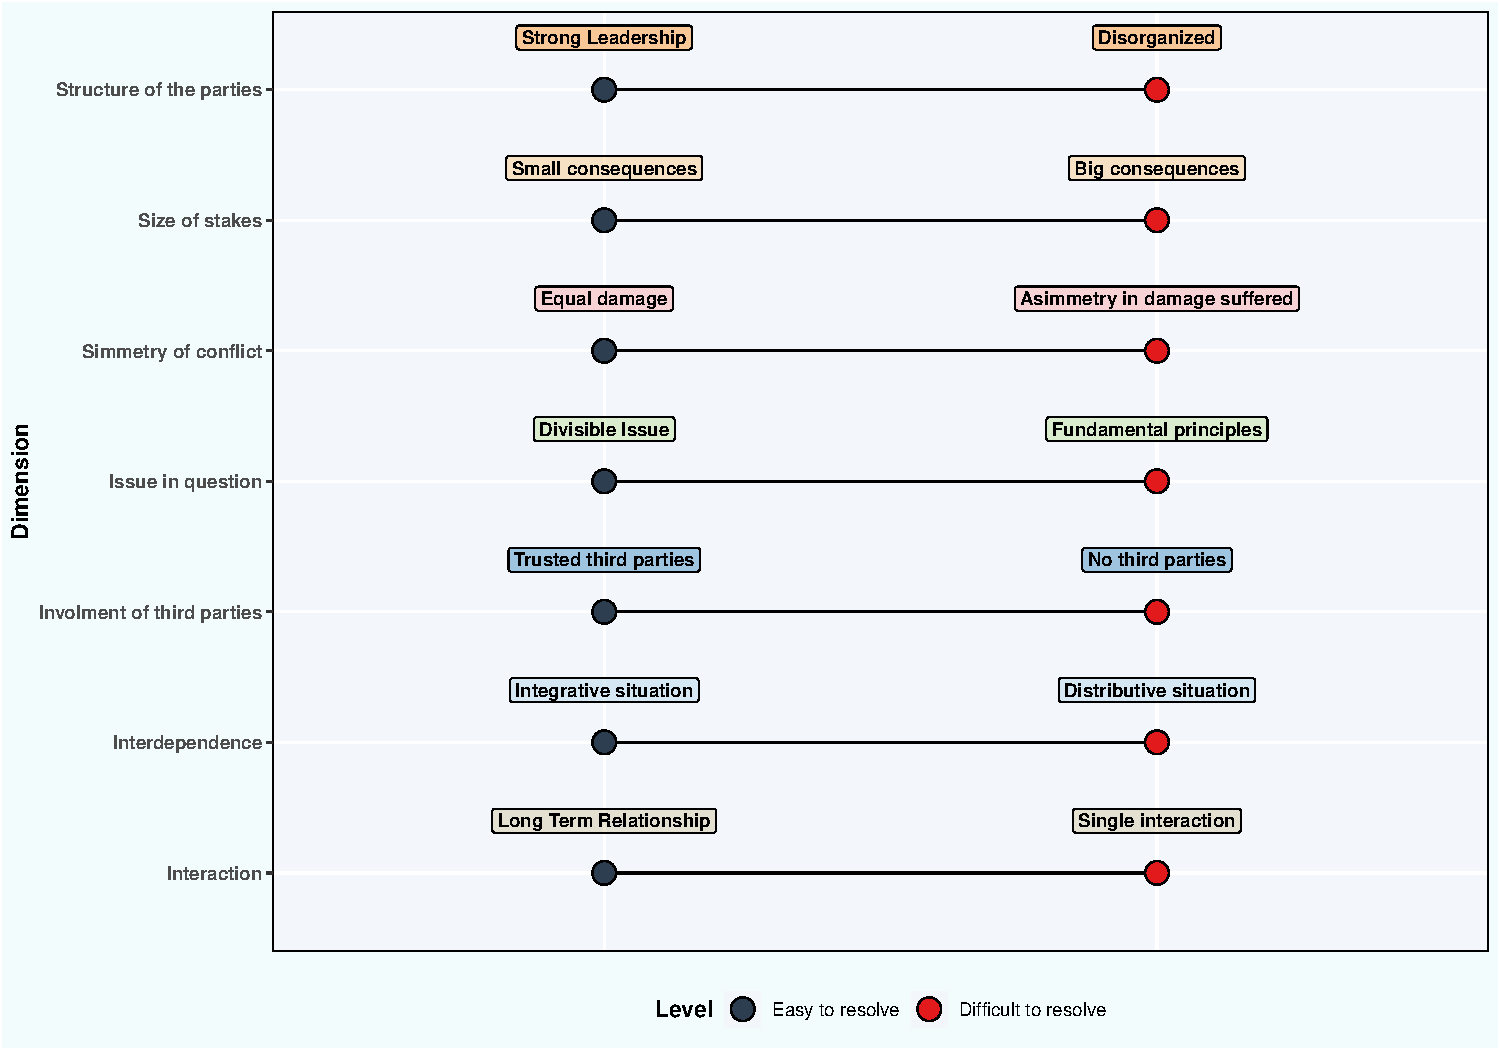
\includegraphics[width=0.85\textwidth,height=\textheight]{001_nature_neg_files/figure-beamer/fig-conflict-diagnostic-model-1.pdf}

}

\caption{\label{fig-conflict-diagnostic-model}Conflict Diagnostic Model
(\citeproc{ref-lewicki_negociacion_2024}{Lewicki, Barry, and Saunders
2024}, p 23) and (\citeproc{ref-greenhalgh_smr_1986}{Greenhalgh 1986}, p
47)}

\end{figure}%
\end{frame}

\section{Effective Conflict
Management}\label{effective-conflict-management}

\begin{frame}{}
\phantomsection\label{section-8}
\begin{figure}

\centering{

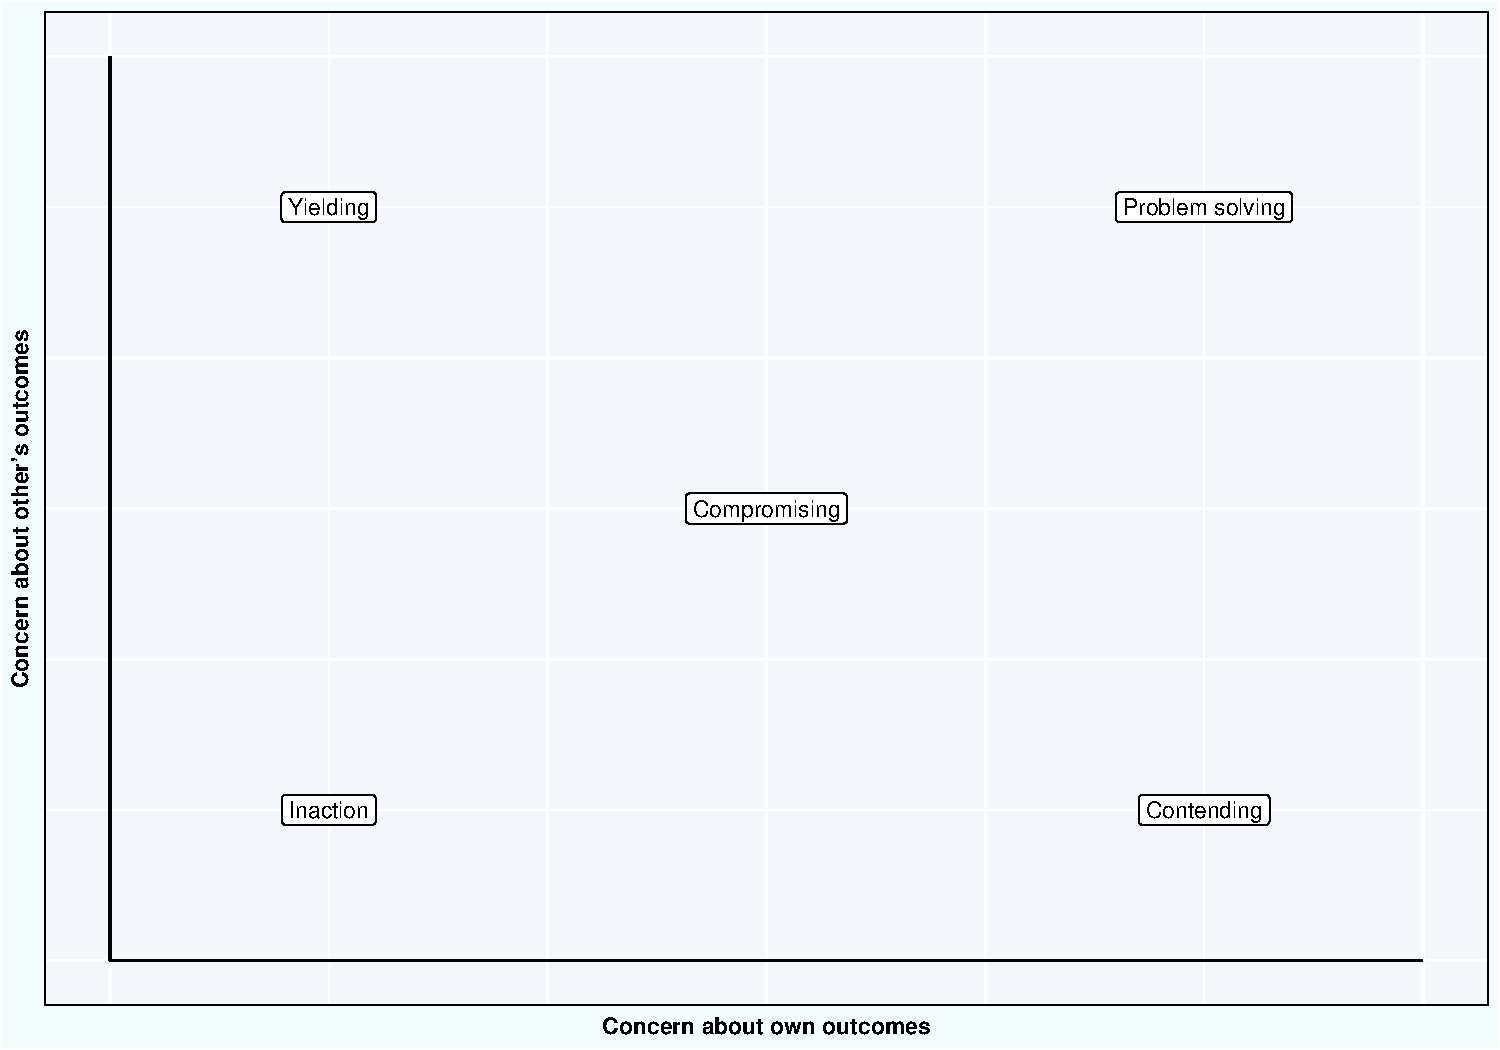
\includegraphics[width=0.85\textwidth,height=\textheight]{001_nature_neg_files/figure-beamer/fig-dual-concerns-model-1.pdf}

}

\caption{\label{fig-dual-concerns-model}Dual concerns model
(\citeproc{ref-lewicki_negociacion_2024}{Lewicki, Barry, and Saunders
2024}, p 24) and (\citeproc{ref-pruitt_social_2004}{Pruitt, Kim, and
Rubin 2004}, p 41)}

\end{figure}%
\end{frame}

\section{Course and book structure}\label{course-and-book-structure}

\begin{frame}{}
\phantomsection\label{section-9}
\begin{itemize}
\item
  Cover in the course

  \begin{itemize}
  \item
    Negotiation Fundamentals

    \begin{itemize}
    \tightlist
    \item
      (\citeproc{ref-lewicki_negociacion_2024}{Lewicki, Barry, and
      Saunders 2024, chaps. 1--5})
    \end{itemize}
  \item
    Negotiation Subprocesses

    \begin{itemize}
    \tightlist
    \item
      (\citeproc{ref-lewicki_negociacion_2024}{Lewicki, Barry, and
      Saunders 2024, chaps. 6--8})
    \end{itemize}
  \item
    Concluding Comments

    \begin{itemize}
    \tightlist
    \item
      (\citeproc{ref-lewicki_negociacion_2024}{Lewicki, Barry, and
      Saunders 2024, chap. 20})
    \end{itemize}
  \end{itemize}
\end{itemize}
\end{frame}

\begin{frame}{}
\phantomsection\label{section-10}
\begin{itemize}
\item
  Not cover in the course

  \begin{itemize}
  \item
    Negotiation Subprocesses

    \begin{itemize}
    \tightlist
    \item
      (\citeproc{ref-lewicki_negociacion_2024}{Lewicki, Barry, and
      Saunders 2024, chap. 9})
    \end{itemize}
  \item
    Negotiation Contexts

    \begin{itemize}
    \tightlist
    \item
      (\citeproc{ref-lewicki_negociacion_2024}{Lewicki, Barry, and
      Saunders 2024, chaps. 10--13})
    \end{itemize}
  \item
    Individual Differences

    \begin{itemize}
    \tightlist
    \item
      (\citeproc{ref-lewicki_negociacion_2024}{Lewicki, Barry, and
      Saunders 2024, chaps. 14--15})
    \end{itemize}
  \item
    Negotiation across Cultures

    \begin{itemize}
    \tightlist
    \item
      (\citeproc{ref-lewicki_negociacion_2024}{Lewicki, Barry, and
      Saunders 2024, chap. 16})
    \end{itemize}
  \item
    Resolving Differences

    \begin{itemize}
    \tightlist
    \item
      (\citeproc{ref-lewicki_negociacion_2024}{Lewicki, Barry, and
      Saunders 2024, chaps. 17--19})
    \end{itemize}
  \end{itemize}
\end{itemize}
\end{frame}

\section{Acknowledgments}\label{acknowledgments}

\begin{frame}{}
\phantomsection\label{section-11}
\begin{itemize}
\item
  To my family that supports me
\item
  To the taxpayers of Colombia and the
  \href{https://www.umng.edu.co/estudiante}{\textbf{UMNG students}} who
  pay my salary
\item
  To the \href{https://www.business-science.io/}{\textbf{Business
  Science}} and \href{https://www.rfordatasci.com/}{\textbf{R4DS Online
  Learning}} communities where I learn
  \href{https://www.r-project.org/about.html}{\textbf{R}} and
  \href{https://www.python.org/about/}{\textbf{\(\pi\)-thon}}
\item
  To the \href{https://www.r-project.org/contributors.html}{\textbf{R
  Core Team}}, the creators of
  \href{https://rstudio.com/products/rstudio/}{\textbf{RStudio IDE}},
  \href{https://quarto.org/}{\textbf{Quarto}} and the authors and
  maintainers of the packages
  \href{https://CRAN.R-project.org/package=tidyverse}{\textbf{tidyverse}},
  \href{https://CRAN.R-project.org/package=tidyquant}{\textbf{tidyquant}},
  \href{https://CRAN.R-project.org/package=ggnewscale}{\textbf{ggnewscale}}
  and
  \href{https://CRAN.R-project.org/package=tinytex}{\textbf{tinytex}}
  for allowing me to access these tools without paying for a license
\item
  To the \href{https://www.kernel.org/category/about.html}{\textbf{Linux
  kernel community}} for allowing me the possibility to use some
  \href{https://static.lwn.net/Distributions/}{\textbf{Linux
  distributions}} as my main
  \href{https://en.wikipedia.org/wiki/Operating_system}{\textbf{OS}}
  without paying for a license
\end{itemize}
\end{frame}

\section*{References}\label{references}
\addcontentsline{toc}{section}{References}

\begin{frame}[allowframebreaks]{References}
\phantomsection\label{refs}
\begin{CSLReferences}{1}{0}
\bibitem[\citeproctext]{ref-greenhalgh_smr_1986}
Greenhalgh, Leonard. 1986. {``{SMR} {Forum}: {Managing} {Conflict}.''}
\emph{Sloan Management Review} 27 (4): 45--51.

\bibitem[\citeproctext]{ref-lewicki_negociacion_2024}
Lewicki, Roy J., Bruce Barry, and David M. Saunders. 2024.
\emph{Negociación}. 9th ed. McGraw-Hill Education.
\url{https://www-ebooks7-24-com.ezproxy.umng.edu.co/?il=40562}.

\bibitem[\citeproctext]{ref-magic_markers_como_2018}
Magic Markers. 2018. {``¿{Cómo} Negociar Bien?''}
\url{https://youtu.be/CnF26cfIfQM}.

\bibitem[\citeproctext]{ref-program_of_negotiation_batna_2012}
Program of Negotiation. 2012. {``{BATNA} {Basics}: {Boost} {Your}
{Power} at the {Bargaining} {Table}.''}
\url{https://www.bc.edu/content/dam/files/centers/cwf/individuals/pdf/BANTABasics.pdf}.

\bibitem[\citeproctext]{ref-pruitt_social_2004}
Pruitt, Dean G., Sung Hee Kim, and Jeffrey Z. Rubin. 2004. \emph{Social
Conflict: Escalation, Stalemate, and Settlement}. 3rd ed.
{McGraw}-{Hill} Series in Social Psychology. Boston: McGraw-Hill.

\bibitem[\citeproctext]{ref-spangler_creating_2003}
Spangler, Brad. 2003. {``Creating and {Claiming} {Value}.''} Conflict
Information Consortium, University of Colorado, Boulder.
\url{https://www.beyondintractability.org/essay/creating_value}.

\end{CSLReferences}
\end{frame}




\end{document}
